This chapter explains about the major tasks implemented in the thesis and new contributions made to the PUF Toolkit. The first part of the chapter briefly explains about the current PUF toolkit implementation, without delving much into the details. This is followed by an explanation of the Hamming Distance Menu which was implemented as a new menu item combining the Intra and Inter-Hamming Distance under one menu. The third part talks about the new modifications that were done to the toolkit in the form of BCH fuzzy extractor encoder and decoder integration, which were previously not a part of the main toolkit and presented as separate executables
with separate menu items. We then go on to explain the Golay code implementation both the decoder and encoder and explain their integration in the toolkit as a distinct menu item. Then the other modifications like the addition of \emph{'offsets from beginning and end', error codes} and other intricate code development changes are presented together as one section. After this, a new metric called \emph{Jaccard Index} is introduced and its implementation along with \emph{Intra and Inter
Jaccard Index} is explained in detail.\\

The final two sections deal with CogniCrypt details and the Java Native Interface (JNI), they first touch upon the basics of JNI
wrapper and the functioning of JNI with shared libraries packaged as JAR files that are accessible to Java compiler as an external library. Finally, we describe the clafer model of the CogniCrypt and how it assists users and Java developers, without any previous knowledge about cryptography, to select a strong PUF based secure key evaluation algorithm based on the questions asked by the CogniCrypt. In the end of this last section, we also talk about the XSL model of the CogniCrypt that builds on
the clafer model to generate a boilerplate Java code to help the Java developer by presenting him/her with a sample use case of the Java code implementation showing a usage of the PUF evaluation algorithms that are robust and flawless.\\

For the implementation, the ISO standardize programming language C++ was chosen. This selection was made based on the efficient and general purpose features provided by C++. Apart from the object-oriented and generic programming features, C++ has a high abstraction level and the compilation and code development can be done on diverse systems. The implementations are dissociated from a specific hardware to support a wide range of systems and applications. This makes the toolkit easier
to extend and conform to a particular hardware for next iterations. The JNI framework support native calls and the wrapper is written in Java, for clafer model we use Javascript and json files along with the .cfr clafer extension modeling language \cite{clafer} and XSL model to generate sample Java boilerplate code is written in XSL.\\

\section{PUF Toolkit}
The current implementation of the PUF toolkit was done and presented in the thesis \cite{71}. The main aim of the toolkit is to evaluate various PUF response based on well-established metrics and thereby helping researchers and designers to gain useful insights into the properties and behavior of PUF responses. The toolkit implements the following list of metrics:

\begin{itemize}
	\item (Shannon) Entropy
	\item Hamming Weight
	\item Intra-Hamming Distance
	\item Inter-Hamming Distance
	\item Min-entropy
	\item Median and average
\end{itemize}

These metrics are thoroughly explained in Sebastian's Master thesis \cite{71}, so we take the liberty to not go into the detail of explaining each metric here again. It must also be noted that there are other metrics and definitions that use identical concepts and/or apply the metrics in a different way to generalize the correlation between different PUF instances and their responses. More exhaustive and comprehensive information related to these metrics and definitions for PUFs can be found in \cite{60,64,24,61}.\\

Apart from the above-mentioned metrics implementation, the PUF based secure key storage is implemented already, using BCH encoder and Decoder in two separate executables. The structure and the User design used in these two executables is similar to the PUF toolkit and to avoid confusion we shall refer to them as \emph{PUF-BCH encoder} and \emph{PUF-BCH decoder}.\\

\subsection{User Design}

The notion of the console user interface was inspired from Nielsen and Molich's nine user interface design guidelines \cite{67}. These guidelines and their resulting effects are shown Table \ref{tab:guidline_design} below:

\begin{table}[!ht]
\begin{center}
\begin{tabular}{cll}
\toprule
\multicolumn{1}{c}{\textbf{No.}} &\multicolumn{1}{c}{\textbf{Guideline}} & \multicolumn{1}{c}{\textbf{Effect}}\\
\midrule
\hline
1 & Simple and natural dialogue & Clear and logical dialogue structure\\

2 & Speak the user’s language & Clear instructions\\

3 & Minimize the user’s memory load & Clean design, brief help and guide texts\\

4 & Be consistent & Consistent design in all menus\\

5 & Provide feedback & Provide feedback and status\\

6 & Provide clearly marked exits & Provide ``back’’ and ``exit’’ in each menu\\

7 & Provide shortcuts & Inputs by abbreviations \\

8 & Good error messages & Provide useful error messages\\

9 & Prevent errors & Handle wrong inputs \\
\hline
\addlinespace
\bottomrule
\end{tabular}
\end{center}
\caption{The nine design guidelines according to \cite{67} and the effect on the UI design.}
\label{tab:guidline_design}
\end{table}

The design of the menu and the (sub-) menus is consistent and recurses itself to make the user interface more intuitive and friendly. Each menu option is written in clear and easy to understand instructions and the menu items are precisely structured to help the user navigate the toolkit with ease. The organization of the menu follows a hierarchical design and a ``back'' function is provided for the user to go to the parent menu. A conceptual depiction of the User Interface is shown in Figure
\ref{img:gui_design}. The Graphical User Interface (GUI) is subdivided into four parts, the color markers are related to the illustration in \ref{img:gui_design}.

\begin{itemize}
	\item The first part, marked in yellow, is the \emph{header}. It gives the user general information, like the title of the current (sub-) menu or brief instructions.
	\item The second part of the gui shows the options and functions that the user can choose from the (sub-) menu, the number in front must be input by the user in the last part of the GUI. The conceptual illustration of the part is marked in red and is called as \emph{Menu}.
	\item Below the Menu part there is \emph{settings and results} that are marked in blue. It shows the current configuration and provides the user with essential information that is vital for the actual computation of the main function. It also shows the output after the computation is performed in the result part of this section.
	\item The fourth part of the GUI is for \emph{feedback} and inputs and is marked in green. It presents the user with the actual processing status, or if an error occurred and the type of the error. Also, it contains a user interactive input cursor, a number must be typed in by the user in order to select the options/functions from the second part, Menu of the GUI.
\end{itemize}

\begin{figure}
\centering
\fbox{ 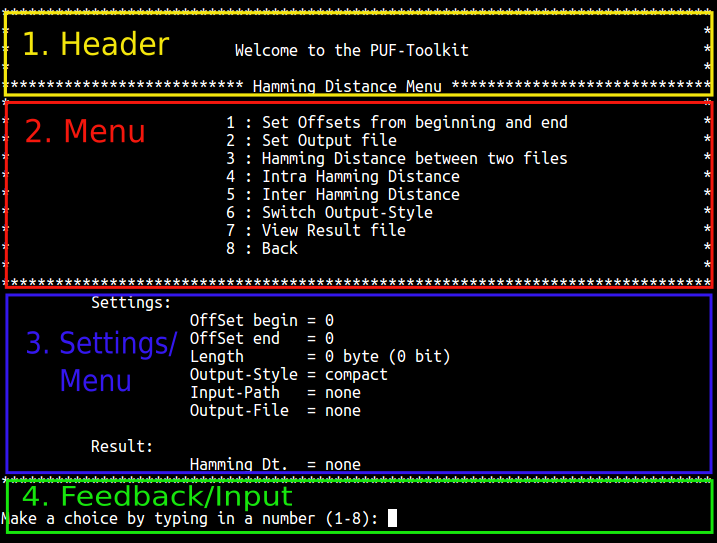
\includegraphics[width=0.9\textwidth]{images/toolkit_gui4.png}}
\caption{Conceptual design of the PUF Toolkit user interface.}
\label{img:gui_design}
\end{figure}

The design of the GUI is kept simple without the use of extended graphic components to keep the toolkit compatible with other operating systems like Linux. The UI shows only relevant information depending on the current state of the program and portrays a simple but aesthetic clean design. Error correction and incorrect user input is efficiently handled, all possible inputs are exhausted and depending on the false input, meaningful errors information is displayed to the user, that can be used to
recover from the erroneous state. Also for all mandatory inputs, a brief guide/help text with examples is shown, the current settings are saved and kept in each (sub-) menu (wherever applicable) to avoid unnecessary redundant input.\\

Rigorously complying with the standardized design guidelines for the toolkit, resulted in a effective and intuitive console user interface.
This in turn decisively supports developers and researchers in the PUFs responses evaluation.\cite{71}

\begin{figure}
\centering
\fbox{ \includegraphics[width=0.97\textwidth, height=\textwidth, keepaspectratio]{images/PUF_Toolkit.pdf}}

\caption{Heirarchical Structure of the PUF Toolkit menu and available options}
\label{img:puf_menu}
\end{figure}

\section{Hamming Distance Menu}
\label{Hamming_Distance_menu}
The hamming distance functionality was added to and integrated as part of this Master thesis. Hamming Distance between two ``bit strings'' of the same length is defined as the number of the bits that differ amongst the two binary bit strings. For eg., if we have two string \emph{A = 1100} and \emph{B = 1010} then the Hamming Distance between them would be ``\emph{two}'', since the bits at second and third position (starting from the left) differ between these two strings. The implementation of
this functionality is straightforward, using the in-built \emph{bitwise XOR} operation of the ISO C++ standard and then counting the number of ones in the resulting string, which is nothing but calling the hamming distance function on the resultant string.\\

As depicted in Figure \ref{img:gui_design} above there are other options like \emph{Intra Hamming Distance} and \emph{Inter Hamming Distance} in the Hamming Distance Menu, that are organized later as subsections where we explain about the different modes and other options and plausible input values, the user can select from. For now, we direct our attention at the other menu items.\\

The first menu item is related to the \emph{\textbf{Offsets}} that are mandatory for the user to input and the first query that must be answered after the toolkit is run. Since the PUF toolkit is designed for evaluation of PUF responses that are in binary format and not all the data in PUF response binary file is useful for evaluation, the user can manually select how much he/she desires to skip the data (in bytes) from the beginning and the end of the file using this \emph{Offsets} option.
For example, the first $400$ bytes of the PUF response of a (TI) Stellaris LM4F120XL Launchpad Evaluation Kit are used during the booting process and are not random, so they are irrelevant in PUF responses evaluation. This kind of device specific behavior requires suitable handling to ensure valid results.\\

Consequently, the \emph{Offset} determines the selection range of the bytes from the PUF response for calculation and also establishing the actual \emph{length} of the response. For eg. if a PUF response is 32784 bytes long and we skip 400 from the beginning and 200 from the end, the actual length becomes $32784-600 = 32184$ bytes and the processing start from the $401^{th}$ byte till $32184^{th}$ byte.\\

The result of the Hamming Distance between two PUF responses can be optionally stored in an output file that is set using the option \emph{two}. This is not mandatory if we are evaluating only two files but in cases of Inter/Intra Hamming Distance this option becomes mandatory. Another functionality added to the Hamming Distance and other Functions in the toolkit as well is that of the Fractional Distance. \newline
$\S$\emph{Defintion}: We define \emph{Fractional Hamming Distance} as the Hamming Distance between two PUF
responses divided by their length. For example, if Hamming Distance between two PUF responses each of length 31784 bytes is 10, then their Fractional Hamming Distance would be $ 10 / 31784 = 0.000314624$ (NOTE: the toolkit displays the fractional hamming distance rounded off to 9 digits after decimal).\\

The Hamming Distance can be calculated using option \emph{three} that will ask for the two PUF responses binary filenames and if the path and filenames are correct, the results will be displayed in the fourth part of the GUI. If the output filename was given before then the result is also stored in that file and can be viewed using the option \emph{seven}.\\

In order to understand the code flow and working of the hamming distance function, it is vital to look at the structure \emph{Item} and its data members. This structure is used by other menus in the toolkit to share the current settings and global configurations like Offsets, filenames, paths etc. and thereby reducing the user's effort and memory load. Table \ref{table:item} only highlights the data members and their purpose that are relevant to Hamming Distance Menu. The other data
members, for the time being, are not shown and will be discussed in relevant sections.\\

\begin{table}[!ht]
	\begin{center}
		\begin{tabular}{ll}
			\toprule
			\multicolumn{1}{c}{\textbf{struct \emph{Item}}} & \multicolumn{1}{c}{\textbf{Purpose}}\\
			\midrule
			\hline

			\emph{offset\_begin} & Defines the starting point in a binary file (bytes to skip from beginning)\\

			\emph{offset\_end} & Defines the ending point in a binary file (bytes to skip from end)\\

			\emph{input\_length} & Defines the number of bytes to use \\

			\emph{input\_file\_name} & Defines the name of the first input file (name and path)\\

			\emph{input\_PUF\_name} & Defines the name of the second input file (name and path)\\

			\emph{output\_file\_name} & Defines the name of the output result file (name and path)\\

			\emph{zeros} & Stores the occurrences of 0s in a defined file\\

			\emph{ones} & Stores the occurrences of 1s in a defined file\\

			\emph{frd} & Stores the fractional distance in a defined file\\

			\emph{result} & Stores the result and feedback regarding the calculations\\

			\emph{HD\_error\_pos} & Additional error information \\

			\hline
			\addlinespace
			\bottomrule
		\end{tabular}
	\end{center}
	\caption{Definition of the elements of the data structure \emph{Item} and their purpose.}
	\label{table:item}
\end{table}

The four lines of code form the basic building block for hamming distance as shown in listing \ref{lst:hammingdt}. First the data is read from the two input PUF files into two arrays of size \emph{dsize} where dsize is equal to the length of the files after applying the Offsets, then as depicted in lines 3-5 of listing \ref{lst:hammingdt} each byte of the data are bitwise XORed and the result is stored in a third array of same length. So the resultant data array contains
\emph{ones} in the position where bits differ in the two PUF responses. We then just need to count the number of ones in the XORed result.
This is done by calling the function \emph{hammingwt} abbreviated in the code for Hamming Weight.\\

\begin{center}
\begin{minipage}{0.7\textwidth}
\begin{lstlisting}[frame=single,language=C++,
commentstyle=\color{green},
backgroundcolor=\color{gray},
keywordstyle=\color{blue},
stringstyle=\color{orange},
basicstyle = \ttfamily \color{black} \footnotesize,
caption={Hamming Distance calculation using hamming weight and bitwise XOR operator} ,
label={lst:hammingdt},
captionpos=b,
numbers=left]
    //bitwise XOR f1data and f2data
    //to get the positions where bits differ
    for (i = 0; i < dsize; i++) {
        data[i] = f1data[i] ^ f2data[i];
    }
    //calculate hamming distance
    item->ones = hammingwt(data, dsize);
    item->frd = (float) item->ones / dsize;
\end{lstlisting}
\end{minipage}
\end{center}

Hamming Weight is one of the essential function of the toolkit and it is also referred to by other functions it's important that we list the code here. Listing \ref{lst:hammingwt} shows the Hamming Weight function as implemented in the toolkit, it takes the data array as a character pointer and its size as arguments. The for loop in lines 5-14 takes each byte of the data and then bitwise ANDs with each bit position (total 8 bit-positions) to count the total occurrences of ones in the byte. This process is
iterated for the entire length ``size'' of the array, each time incrementing the counter ``wt'' whenever a one is encountered and finally, the hamming weight is returned to the caller function.\\


\begin{center}
\begin{minipage}{0.7\textwidth}
\begin{lstlisting}[frame=single,language=C++,
commentstyle=\color{green},
backgroundcolor=\color{gray},
keywordstyle=\color{blue},
stringstyle=\color{orange},
basicstyle = \ttfamily \color{black} \footnotesize,
caption={Hamming Weight calculation using bitwise AND operator} ,
label={lst:hammingwt},
captionpos=b,
numbers=left]
int hammingwt(char *data, int size)
{
    int i;
    int wt = 0;
    for (i = 0; i < size; i++) {
        (data[i] & 0x80 ? wt++ : wt); //8th bit position
        (data[i] & 0x40 ? wt++ : wt); //7th bit position
        (data[i] & 0x20 ? wt++ : wt); //6th bit position
        (data[i] & 0x10 ? wt++ : wt); //5th bit position
        (data[i] & 0x08 ? wt++ : wt); //4th bit position
        (data[i] & 0x04 ? wt++ : wt); //3th bit position
        (data[i] & 0x02 ? wt++ : wt); //2nd bit position
        (data[i] & 0x01 ? wt++ : wt); //1st bit position
    }
    return wt;
}
\end{lstlisting}
\end{minipage}
\end{center}

\subsection{Intra-Hamming Distance}
\label{intra_hd_section}
This section explains the Intra-Hamming Distance feature which is a comparison of the PUF responses from the same device. As discussed in section \ref{intra_inter_section} we already observed that the PUF responses from the same device are not identical due various factors like voltage fluctuation,  temperature variation, and other aging effects, which gives rise to Intra distance within the responses. ``Intra'' means on the inside, so we evaluate the PUF instance from within by assessing the Hamming Distance within
these responses. Since the hardware from which the SRAM PUFs are obtained are kept in a single directory, we need only to give the ``input path'' for processing Intra Hamming Distance, the output file option is mandatory to process Intra HD because the results must be stored for all the responses in a file to be viewed later. Along with the Hamming Distance between PUF responses the fractional distance is also saved for better assessment of the PUF instance.\\

A crucial attribute in the ``Switch output-style'' which can be used to change the save format of the output file, there are two possibilities for Intra HD: \emph{compact} and \emph{minimal}. The compact mode takes each file in the directory and recursively compares with all the other files, then the second file is chosen and compared with the all the other except the first one and so on. The fig. \ref{img:4_intra_WP} illustrates this comparison.  The output style ``\emph{compact}'' is the default format style and should be used
as an output format for a regular text file. Due to the symmetrical behavior of the comparison ( A to B = B to A), we need not exhaust all 1-to-1 possible combinations. So in compact mode first entry from the directory is compared to all the other till the last entry, then the second entry is compared to the third entry till last file, then the third with fourth entry and so on till we are at the last file which need not be compared to any of the above entries since we have already exhausted the
symmetric comparisons.\\

\begin{figure}
\centering
\fbox{ \includegraphics[width=0.9\textwidth]{images/intra_compact.pdf}}
\caption{Visualization of the \emph{compact} output style format for Intra Hamming Distance.}
\label{img:4_intra_compact}
\end{figure}

\begin{figure}
\centering
\fbox{ 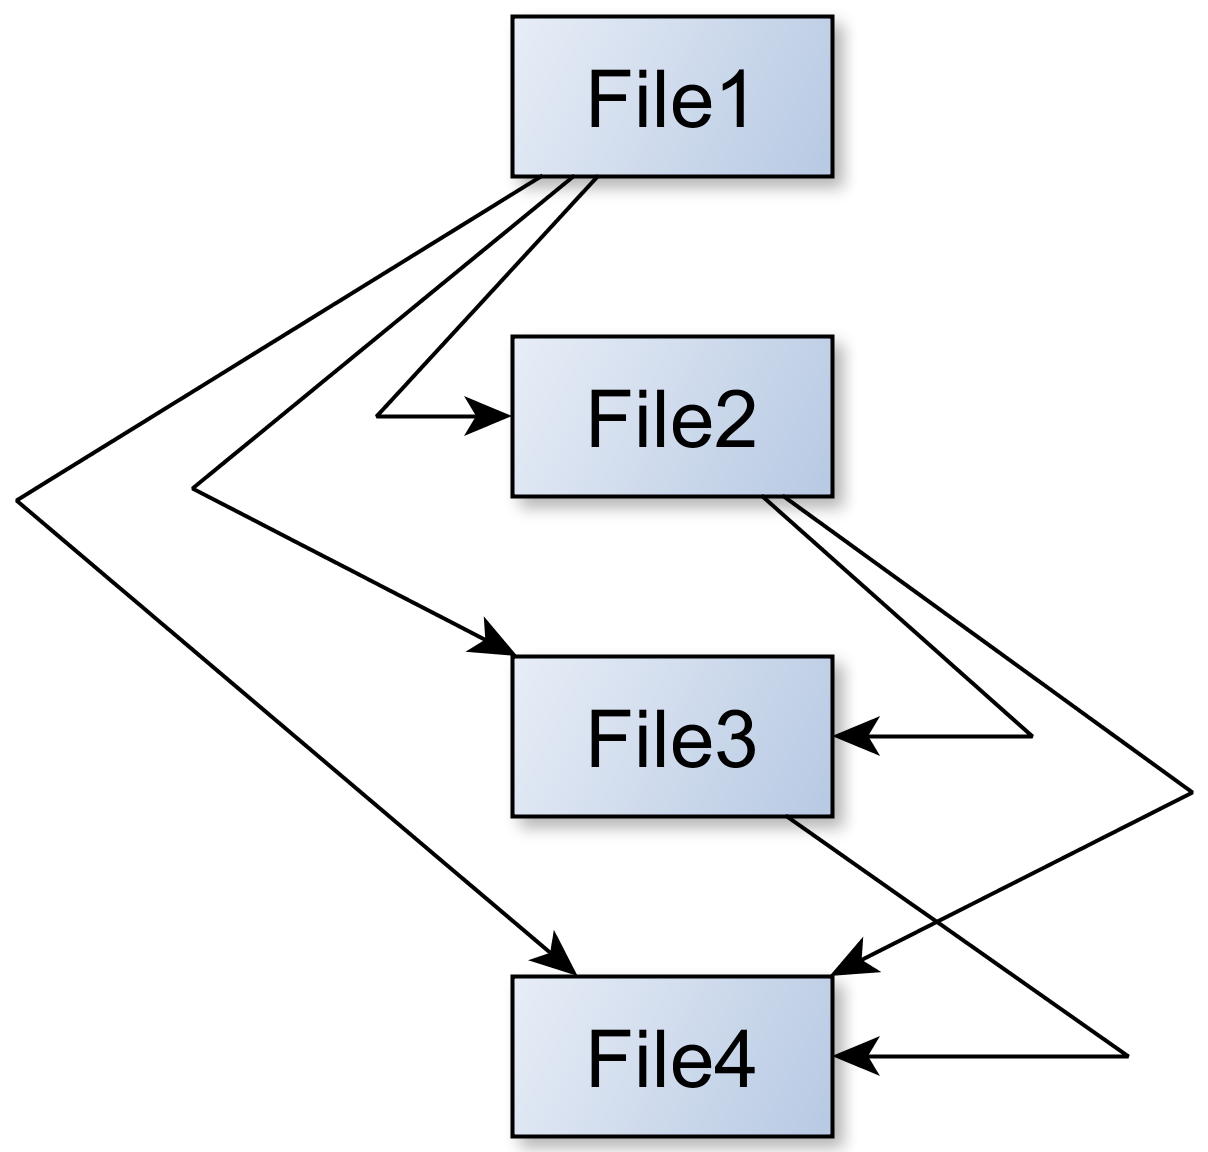
\includegraphics[width=0.4\textwidth]{images/Intra.png}}
\caption{Exemplary illustration of the working principle of the \emph{compact} mode, for the intra-Hamming distance.}
\label{img:4_intra_WP}
\end{figure}

A sample output file with compact style format is shown in Figure \ref{img:4_intra_compact} that evaluates the PUF instance from a single directory using Intra Hamming Distance metric, it also appends the fractional distance information to the file. It consists of a header with general information that shows the configuration (like offsets, device folder etc.) that was used for evaluation and three tables. In the upper right corner of each table the utilized input file is shown and on the left side of the table
the files, that are compared to the selected input file, are displayed. The Hamming Distance and Fractional Hamming Distance, separated by a tab length are printed in the center (right) of each table. The
\emph{minimal} output style strips off all the path and filename info and only saves the Hamming Distance values separated by spaces, this type of file format can be used by another metric of the toolkit called Median and Average calculation (section 4.1 \cite{71}) which accepts only files containing plain numbers separated with space. The \emph{View} option can be used to look at the output/result file.\\

\subsection{Inter Hamming Distance}
\label{inter_hd_section}
Contrary to the comparisons between PUF responses from the same device, Inter Hamming distance evaluates responses from different PUF instance. The co-relation is again based on the same metric Hamming Distance. In this case, the toolkit can simultaneously compare from 2 to 99 PUF instances. All the PUF responses from a specific instance are arranged in a single directory so that means the toolkit can take input paths between 2 and 99 to evaluate different PUF devices. The output
style in addition to compact and minimal has a \emph{detailed} as an alternative. The compact and minimal style formats are same as Intra Hamming Distance, but the detailed style differs from the compact style that it does not implicitly ignores the duplicate symmetric comparisons and therefore maps out all the permutations and combinations between files of different folders. It should be noted that Inter Hamming Distance metric does not compare PUF responses in the same directory. So
in detailed mode, the first directory all the responses are compared to all the PUF responses from the remaining 3 to 99, then all files in the second folder are compared to all the files in all the other folders except its own, and so on. Figure \ref{img:inter_output} shows a sample output with 3 input paths, for compact mode we need to ignore the duplicate comparisons so we take the following approach:
\begin{itemize}
	\item store all the filenames and their corresponding paths from all but last folder in list1.
	\item store all the filenames and their corresponding paths from all but the first folder in list2.
	\item iterate over list1 (iteration 1-4) and compare the list1 objects with all entries of list2.
	\item remove the second folder objects from list2.
	\item iterate over list1 (iteration 5-7) and compare the list1 objects with all files of list2.
\end{itemize}

\begin{figure}
\centering
\fbox{ \includegraphics[width=0.97\textwidth]{images/inter_compact.pdf}}
\caption{A sample output showing the visualization of the inter hamming distance \emph{compact} output style format.}
\label{img:inter_output}
\end{figure}

\begin{figure}
\centering
\fbox{ 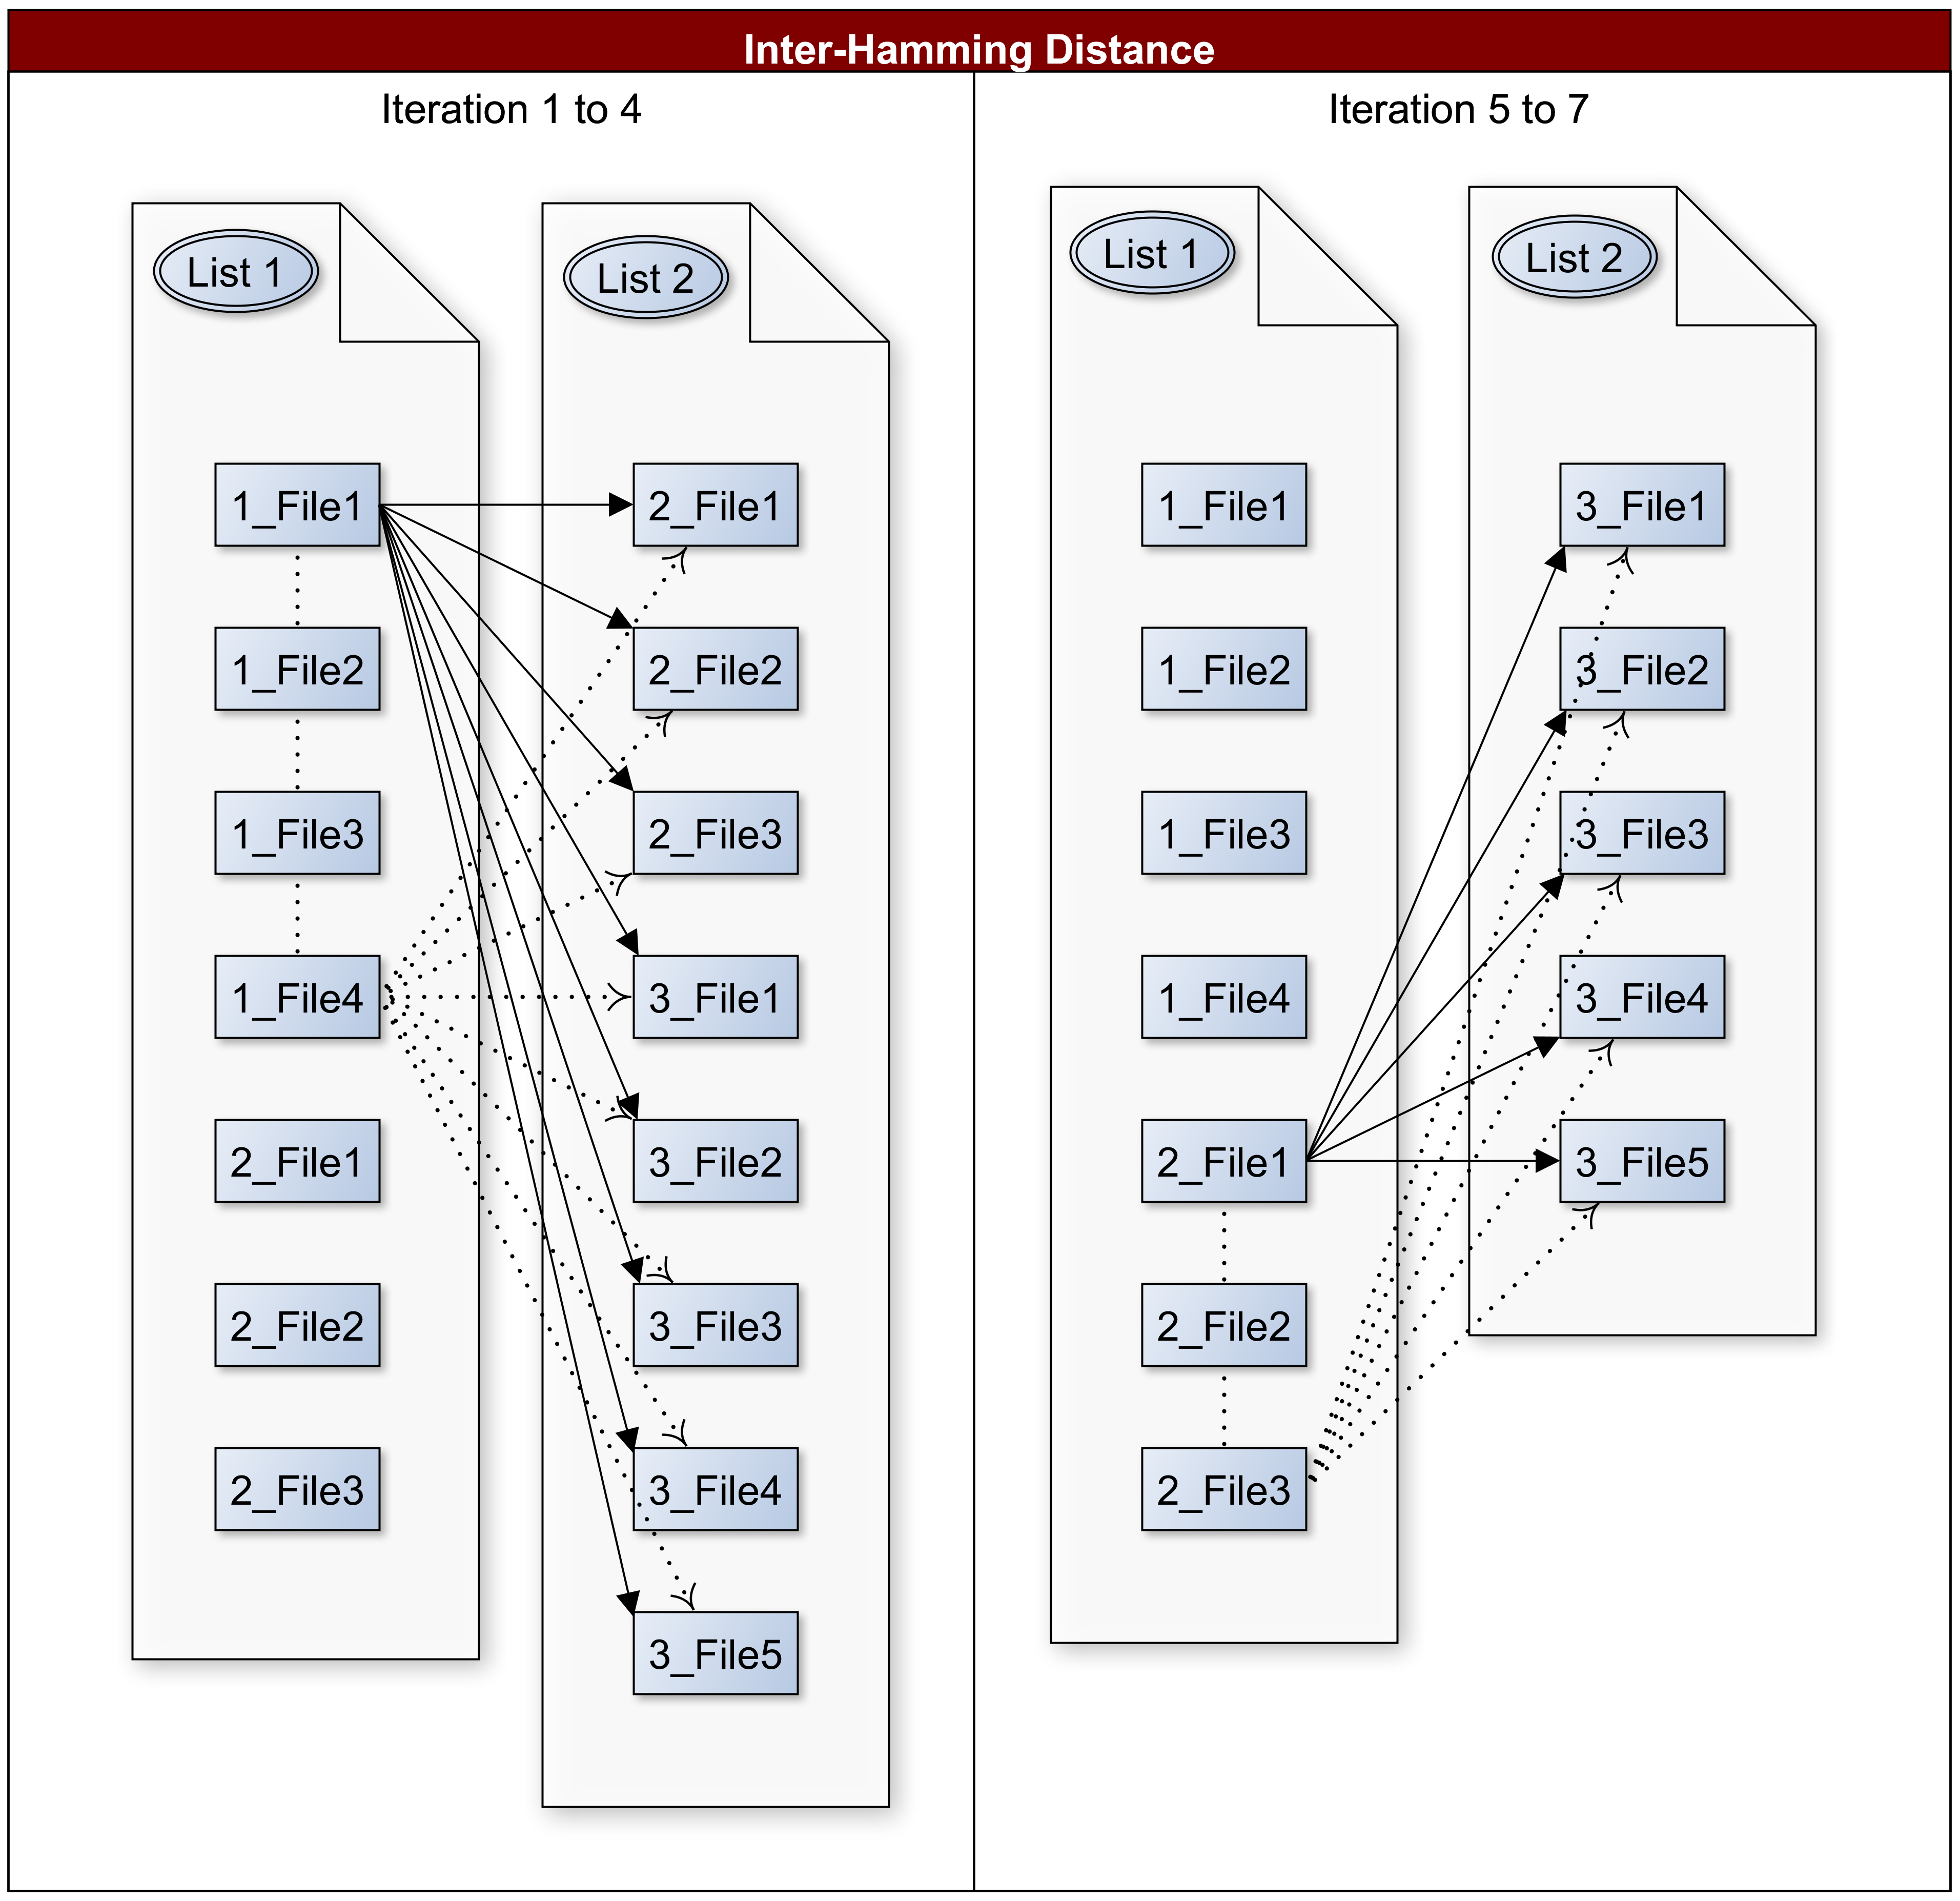
\includegraphics[width=0.97\textwidth]{images/Inter_itr.png}}
\caption{Exemplary illustration of the working principle of the \emph{compact} mode, for the intra-Hamming distance.}
\label{img:inter_compact}
\end{figure}

This process is summarized in Figure \ref{img:inter_compact} for three folder input and is generalized for more inputs. We emphasize on the inner workings of the modes because the exact same techniques are used for Jaccard's index that will be discussed later in this chapter.\\

\emph{Menu Modifications:} In contrast to the original toolkit where Intra and Inter Hamming Distance were separated in their own sub-menus, the new changes merge both of them under Hamming Distance Menu. Seeing as it is relevant to combine them if they use the same underlying metric, on the other hand, the Hamming Weight menu item was untouched since it takes only one PUF response file as an input and gives out its hamming weight and there is no evaluation between two or
more files.\\


\section{Fuzzy extractor}
As discussed in section \ref{fuzzy_section} the PUF based secure key storage uses Fuzzy Extractor technique that is divided into three phases \emph{(i)Pre-evaluation}, \emph{(ii) Enrollment} and \emph{(iii) Reconstruction}. The second and third phase follow a separate implementation of the respectively dedicated functionalities, according to \cite{10}. The enrollment phase is presented with the help of an Entity Relation Diagram. Similar to BCH encoder
section we examine the changes required during merging with the toolkit in the subsection ``Integration Changes'' and finally talk about the verification steps taken to assert the correctness of the merged decoder functionality in the toolkit.\\UF BCH encoder which will be discussed first followed by the Reconstruction phase, that is
realized by the PUF BCH Decoder implementation. We will not go into the details of the actual implementation of the encoder and decoder since they are already well documented in \cite{71}, but rather explain the changes made to integrate these functionalities in the PUF toolkit.\\

The concept of fuzzy extractor in combination with BCH coding with linear repetition code and majority voting is depicted in Figures \ref{img:4_BCH_concept}, \ref{img:4_LR_HD} and \ref{img:4_MV_codewords}.

\begin{figure}[h]
\centering
\fbox{ 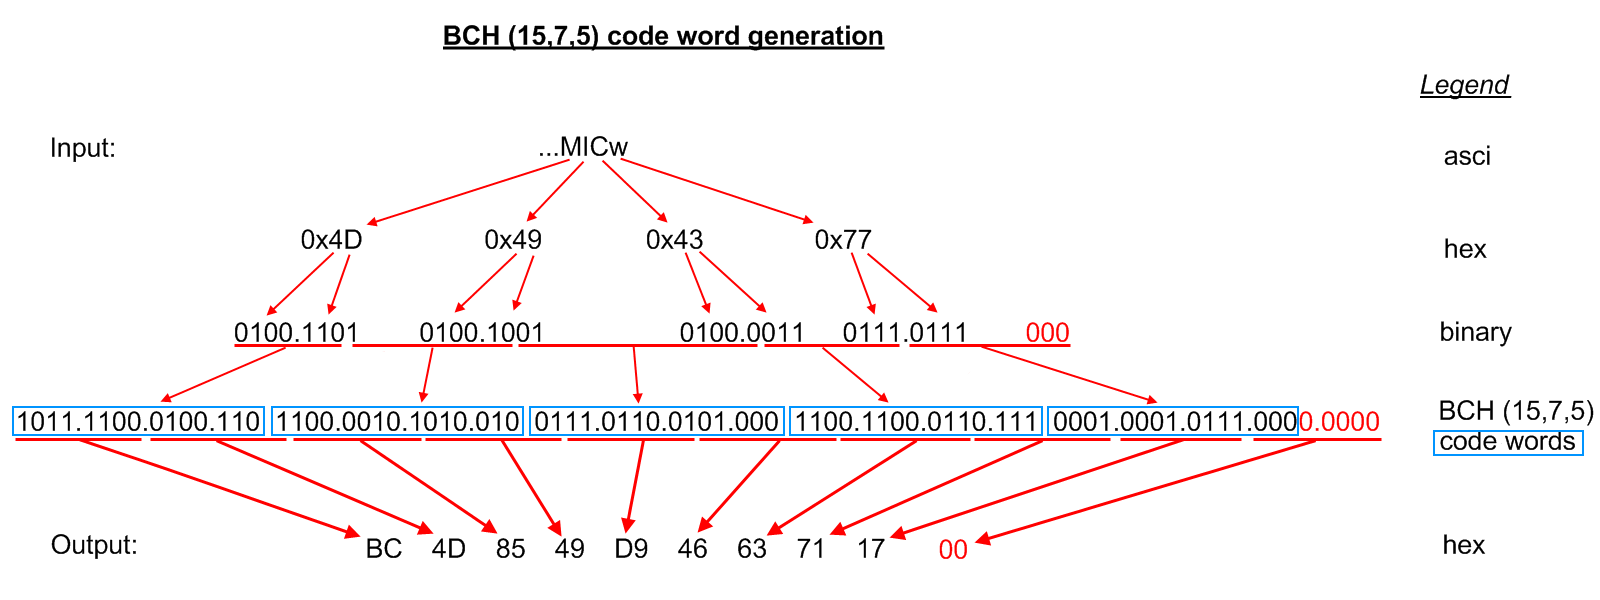
\includegraphics[width=0.97\textwidth]{images/BCHconcept.png}}
\caption{Exemplary code word generation with a BCH (15,7,5) code, based on \cite{10}.}
\label{img:4_BCH_concept}
\end{figure}

\begin{figure}[h]
\centering
\fbox{ 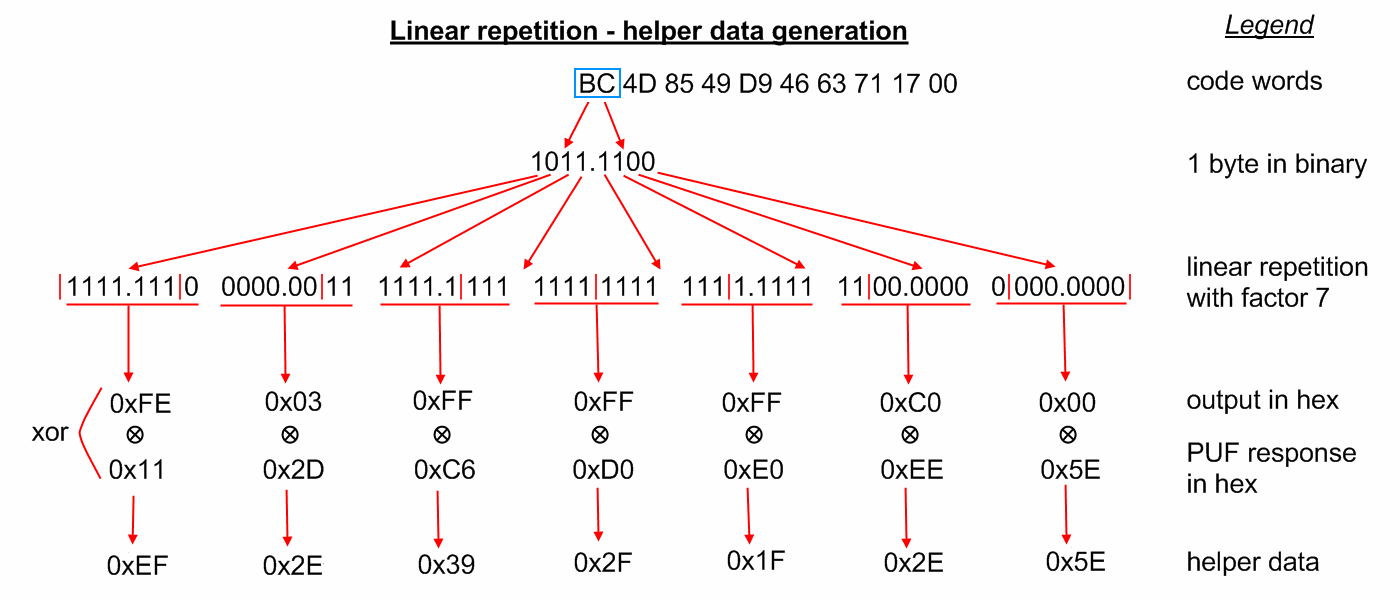
\includegraphics[width=0.97\textwidth]{images/LRhd.png}}
\caption{Exemplary helper data generation with a linear repetition code and factor 7, based on \cite{10}.}
\label{img:4_LR_HD}
\end{figure}

\begin{figure}[h]
\centering
\fbox{ 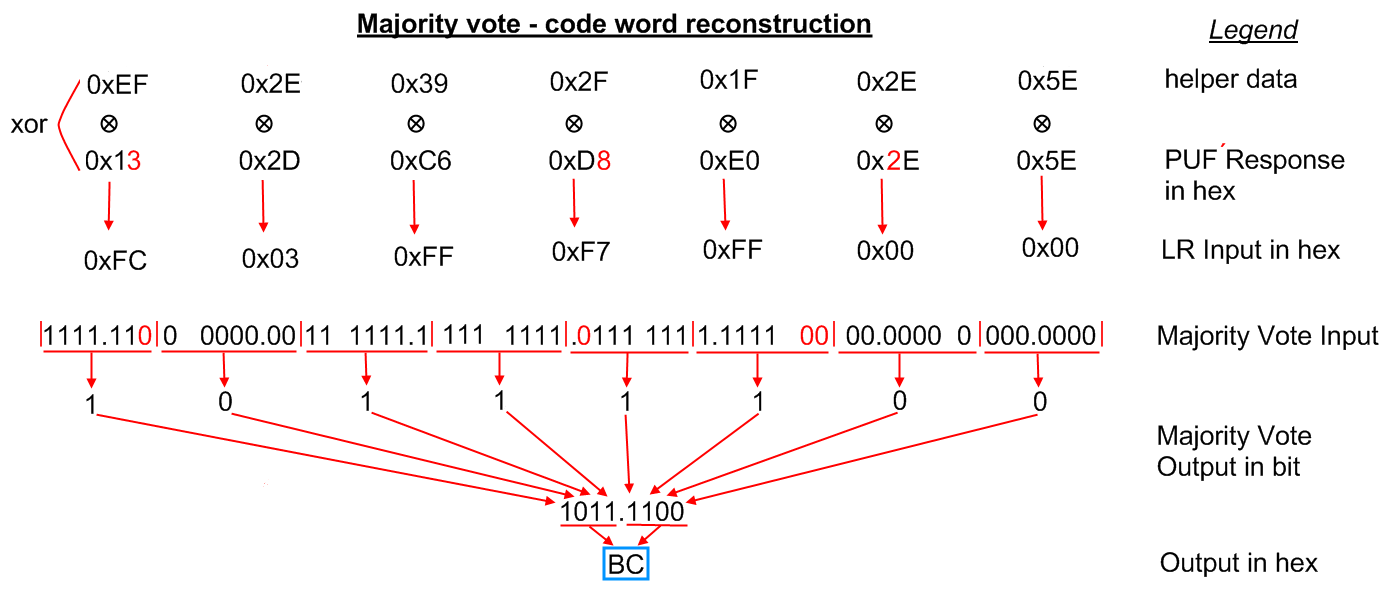
\includegraphics[width=0.97\textwidth]{images/MVrecon.png}}
\caption{Exemplary code word reconstruction with the majority vote and factor 7, based on \cite{10}.}
\label{img:4_MV_codewords}
\end{figure}

\subsection{PUF BCH Encoder}
This section first briefly mentions the implementation algorithm used in the BCH encoding of the data, after that the user interface is illustrated followed by an Entity Relation Diagram that shows major functions of the encoder. The changes are presented as a subsection named integration changes and the section is concluded by showing the steps taken to verify the integrated BCH encoder.\\

The BCH encoding implementation is taken from \emph{Morelos-Zaragoza's Encoder/Decoder} for binary BCH codes in C \cite{69}. This algorithm uses systematic encoding to encode the message, hence the encoded codewords contain initial message in it, which is stripped from the codeword to get the helper data, using the BCH(n,k,d) (refer section \ref{bch_section}) the codewords are combined in groups of \emph{length k} and extra 0s are added to complete the last set. In the
second part of the enrollment of the fuzzy extractor, the LR code is applied to the generated codeword, based on the user input the bits are repeated either 7 or 15 times, Figure \ref{img:4_LR_HD} shows this LR process with factor 7. It was noted that there were some limitations to the original algorithm and the encoding only works for small values of $m$, after code review and research the error states were removed and/or documented.\\

	Due to above-mentioned limitations, the correct combination of BCH encoding and linear repetition code requires correct handling of the bounds. The length of the secret key in bits is denoted by $N$, to process the entire file with BCH (n,k,d) code we need \emph{len} iterations of encoding, this is defined in Equation \ref{4:BCH_len}.

	\begin{itemize}
		\item For an input data of length \emph{N} (bits) and a BCH ($n$,$k$,$d$) code, a ‘\emph{len}’ number of BCH encoding iterations have to be performed to process the complete input file \cite{71}:
	\begin{equation}
		len =\Bigg\lceil\dfrac{N}{k}\Bigg\rceil
		\label{4:BCH_len}
	\end{equation}

	\item For a BCH ($n$,$k$,$d$) code that requires ‘\emph{len}’ BCH encoding iterations to process the complete input file, the result of the linear repetition code has a length of ‘\emph{LengthAfterLR}’ with respect to the chosen linear repetition factor ‘\emph{LRfactor}’ (7 or 15) \cite{71}:
	\begin{equation}
		LengthAfterLR = \Bigg\lceil\Bigg(\dfrac{\Bigg(\dfrac{len}{k} * n\Bigg)}{8}\Bigg)\Bigg\rceil * LRfactor
	\label{4:BCH_LR_len}
	\end{equation}
	\end{itemize}

	\begin{figure}
	\centering
	\fbox{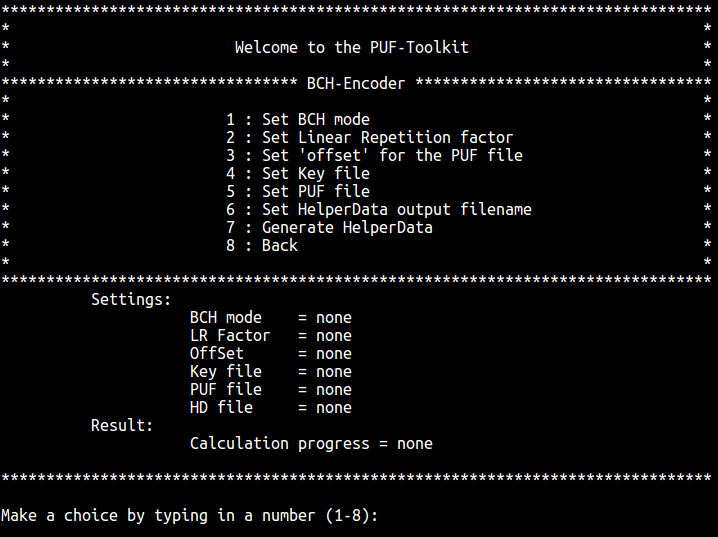
\includegraphics[width=0.9\textwidth]{images/bch_encoder_ui.png}}
	\caption{Console user interface of the \emph{PUF BCH Encoder}.}
	\label{img:4_BCH_ENC_menu}
	\end{figure}
	The User interface for the BCH Encoder sub-menu is shown in Figure \ref{img:4_BCH_ENC_menu}. The first option is to set the BCH mode in which the user is required to input the code length $n$ i.e. derived from $m$ such that $(2^{m-1} - 1) < length <= (2^m - 1)$, after that it is also mandatory to enter the desired correction capability $t$ of the BCH (n,k,d) code that in turn will determine the parameter $d$ of the code from the formula $t = \lfloor(d-1)/2\rfloor$.
	These values must be consistent with the equations \ref{4:BCH_len} and \ref{4:BCH_LR_len} or else the decoding of the secret key will not be successful. The second option chooses the LR factor as 7 or 15, the third is the familiar offsets selection for the PUF response that will also determine the actual length of the PUF response used to generate the helper data. After this the user must also input the key he/she wants to securely store and the name of the PUF
	response file, finally the output filename for helper data must be provided to be saved on permanent storage and to be used in the later reconstruction phase of the fuzzy extraction. These discussed inputs are all mandatory in the BCH menu and only then we can use option seven to process and generate the helper data or else the toolkit throws appropriate error messages to the user about missing parameters.\\

	The functions of the BCH encoder arranged in modules that are related to each other are depicted in Figure \ref{img:bchenc_fns}

	\begin{figure}
	\centering
	\fbox{ \includegraphics[width=0.9\textwidth]{images/bch_encoder_functions.pdf}}
	\caption{Dependencies of the BCH Encoder Modules}
	\label{img:bchenc_fns}
	\end{figure}

	The data structure \emph{Item} that was discussed in Hamming Distance contains relevant data members related to BCH encoder, which is summarized in Table \ref{tab:4_BCH_item_type_limits}

	\begin{table}[!ht]
	\begin{center}
	\begin{tabular}{lll}
	\toprule
	\multicolumn{1}{l}{\textbf{Name}} & \multicolumn{1}{l}{\textbf{Type}} & \multicolumn{1}{c}{\textbf{Description}}\\
	\midrule
	\hline
	\emph{offset\_begin} & long & \multicolumn{1}{l}{\begin{tabular}[l]{@{}l@{}}Defines the starting point in a binary file (bytes to skip from beginning) \end{tabular}}\\

	\emph{offset\_end} & long & \multicolumn{1}{l}{\begin{tabular}[l]{@{}l@{}}Defines the ending point in a binary file (bytes to skip from end) \end{tabular}}\\

	\emph{input\_Key\_length} & long & \multicolumn{1}{l}{\begin{tabular}[l]{@{}l@{}}Defines the length of the input key file\end{tabular}}\\

	\emph{input\_Key\_name} & char [102] & \multicolumn{1}{l}{\begin{tabular}[l]{@{}l@{}}Char array for 102 symbols, to define the input key file \end{tabular}}\\

	\emph{input\_PUF\_name} & char [102] & \multicolumn{1}{l}{\begin{tabular}[l]{@{}l@{}}Char array for 102 symbols, to define the input PUF file \end{tabular}}\\

	\emph{output\_HD\_name} &  char [102] & \multicolumn{1}{l}{\begin{tabular}[l]{@{}l@{}}Char array for 102 symbols, to define the output helper data file \end{tabular}}\\

	\emph{BCHmode} & char [25] & \multicolumn{1}{l}{\begin{tabular}[l]{@{}l@{}}Char array for 25 symbols, to define the BCH mode \end{tabular}}\\

	\emph{LR} & int & \multicolumn{1}{l}{\begin{tabular}[l]{@{}l@{}}Definition of the utilized linear repetition factor \end{tabular}}\\

	\emph{result} & char [52] & \multicolumn{1}{l}{\begin{tabular}[l]{@{}l@{}}Char array for 52 symbols, to provide feedback \end{tabular}}\\
	\hline
	\addlinespace
	\bottomrule
	\end{tabular}
	\end{center}
	\caption{Names and types of each element in the data structure \emph{Item} for the \emph{PUF BCH Encoder} and a description regarding their purpose.}
	\label{tab:4_BCH_item_type_limits}
	\end{table}

	\subsubsection{Integration changes}
	Initially, the BCH Menu item was defined in the toolkit module to be called by the main menu, after that support for Offset from beginning and end, depicted in Table \ref{tab:4_BCH_DEC_item_type_limits}, was made available similar to Hamming Distance menu. Since the ``Calculation module'' functions of the BCH encoder are all called internally without any dependence on the user, so they were unified with the original PUF Toolkit Calculation module without much hindrance.
	The ``Settings module'' was merged to the toolkit with \emph{DefineFilename\_BCH} was renamed to avoid function name conflict with \emph{DefineFilename} of the toolkit, the former is dedicated to processing the input PUF filename, output helper data file and input secret key of the BCH encoder. The ``File and View modules'' were straightforward to unify with the toolkit, special care was taken to add the BCH global variables and global vectors to the toolkit. Changes in the ``View
	module'' were dominated by the \emph{ErrorMessages} routine, which informs the user about the incorrect input and error states and the ways to recover from them. Major challenges faced during the integration were the same name functions as in the original toolkit that resulted in linking errors, they were resolved by renaming them appropriately for BCH encoder and all the declarations of the resulting functions were unified in the header files of the respective modules.\\

	\subsubsection{Verification}
	The correctness after merging the BCH encoder was authenticated via exhaustive run through all the test cases. In addition to that, a final verification of the entire implementation was done. While doing the verification following main points were given priority:

	\begin{itemize}
		\item The correctness of each module verified through utilization of test cases.
		\item All the possible menu options were checked and reviewed for their expected functionality
		\item Wrong inputs were tested to make sure that the toolkit accepts only legitimate inputs and display appropriate error messages to rectify the error.
		\item Unusual workflows were inspected to assess their impact on Encoder functionality.
	\end{itemize}

	\subsection{PUF BCH Decoder}
	We now go on to discuss the second phase of the fuzzy extractor i.e.``regeneration'' that uses PUF BCH Decoder as an essential element to recover the secret key that was encoded in the first phase with the help of the generated helper data and a PUF response from the same device as used in the enrollment phase. Again we do not indulge in the exact implementation details since they are presented in great detail in \cite{71}. This section looks at the user interface of the BCH decoder where the possible inputs and their meaning is discussed, then a summary of the main modules involved in the BCH decoder
	is presented with the help of an Entity Relation Diagram. Similar to BCH encoder section we examine the changes required during merging with the toolkit in the subsection ``Integration Changes'' and finally talk about the verification steps taken to assert the correctness of the merged decoder functionality in the toolkit.\\

	The decoder implementation is also the extension of the Morelos-Zaragoza's code \cite{69} but before applying the decoding functionality, the LR encoded helper data received from the first phase is processed in the majority vote module of the fuzzy extractor as shown in Figure \ref{img:4_MV_codewords}. This counteracts the linear repetition introduced in the LR coding module of the ``enrollment phase''. The fig. \ref{img:4_MV_codewords} shows this operation on the helper data received from fig. \ref{img:4_LR_HD}, notice that the PUF
	response has some bits changed due to the various environmental factors (like temperature change and voltage fluctuation) that introduce intra distance between the PUF responses from the same device. After the Majority Vote operation the BCH decoder recovers the configuration settings \emph{cfg} that are appended to the end of the helper data to satisfy correct boundary conditions as seen in the BCH encoding phase. Usually, the BCH(n,k,d) can correct up to $t$ bit flip errors though along with Majority
	Voting and BCH decoding the fuzzy extractor can restore the original input secret key.\\

	\begin{figure}
	\centering
	\fbox{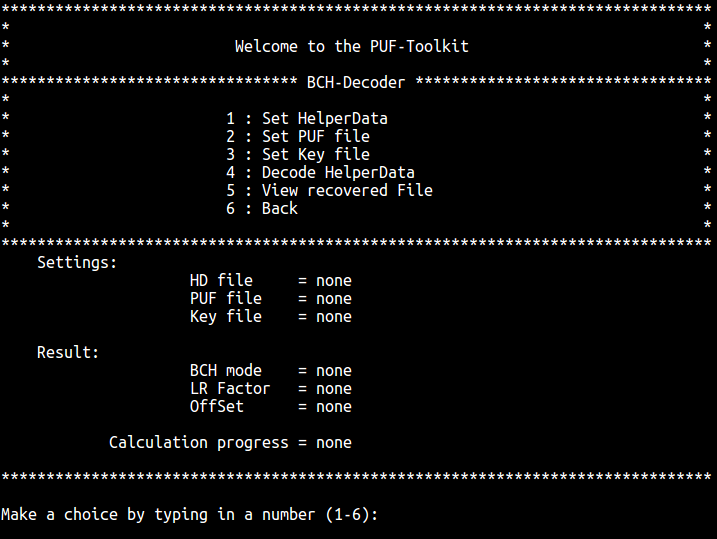
\includegraphics[width=0.9\textwidth]{images/bch_decoder_ui.png}}
	\caption{Console user interface of the \emph{PUF BCH Decoder}.}
	\label{img:BCH_decoder_GUI}
	\end{figure}
	The User interface is a simple GUI similar to the BCH encoder \ref{img:BCH_decoder_GUI}, but in this case, the user need not enter the BCH mode details and offsets since they are predetermined in the encoding part and are saved as \emph{cfg} settings. We only need to give the helper data filename and the PUF response filename to decode and restore the input secret key. The output key filename is required to store the recovered input secret key and using option ``$5$'' the retrieved key can be viewed without
	exiting the toolkit.\\

	The five modules of the BCH decoder and their functions are depicted in Figure \ref{img:bchdec_fns}.
	\begin{figure}
	\centering
	\fbox{ \includegraphics[width=0.9\textwidth]{images/bch_decoder_functions.pdf}}
	\caption{Dependencies of the BCH Encoder Modules}
	\label{img:bchdec_fns}
	\end{figure}

	The members of the data structure \emph{Item} those are relevant to the BCH decoder are summarized in Table \ref{tab:4_BCH_DEC_item_type_limits}. The only difference with the encoder is that we need input helper data filename instead of output helper data filename and output key filename instead of the input key filename.

	\begin{table}[!ht]
	\begin{center}
	\begin{tabular}{lll}
	\toprule
	\multicolumn{1}{l}{\textbf{Name}} & \multicolumn{1}{c}{\textbf{Type}} & \multicolumn{1}{c}{\textbf{Description}}\\
	\midrule
	\hline
	\emph{offset\_begin} & long & \multicolumn{1}{l}{\begin{tabular}[l]{@{}l@{}}Defines the starting point in a binary file (bytes to skip from beginning) \end{tabular}}\\

	\emph{offset\_end} & long & \multicolumn{1}{l}{\begin{tabular}[l]{@{}l@{}}Defines the ending point in a binary file (bytes to skip from end) \end{tabular}}\\

	\emph{input\_HD\_name} &  char [102] & \multicolumn{1}{l}{\begin{tabular}[l]{@{}l@{}}Char array for 102 symbols, to define the input helper data file \end{tabular}}\\

	\emph{input\_PUF\_name} & char [102] & \multicolumn{1}{l}{\begin{tabular}[l]{@{}l@{}}Char array for 102 symbols, to define the input PUF file \end{tabular}}\\

	\emph{output\_Key\_name} & char [102] & \multicolumn{1}{l}{\begin{tabular}[l]{@{}l@{}}Char array for 102 symbols, to define the output key file \end{tabular}}\\

	\emph{BCHmode} & char [25] & \multicolumn{1}{l}{\begin{tabular}[l]{@{}l@{}}Char array for 25 symbols, to define the BCH mode \end{tabular}}\\

	\emph{LR} & int & \multicolumn{1}{l}{\begin{tabular}[l]{@{}l@{}}Definition of the utilized linear repetition factor \end{tabular}}\\

	\emph{result} & char [52] & \multicolumn{1}{l}{\begin{tabular}[l]{@{}l@{}}Char array for 52 symbols, to provide feedback \end{tabular}}\\
	\hline
	\addlinespace
	\bottomrule
	\end{tabular}
	\end{center}
	\caption{Names and types of each element in the data structure \emph{Item} for the \emph{PUF BCH Decoder} and a description regarding their purpose.}
	\label{tab:4_BCH_DEC_item_type_limits}
	\end{table}

	\subsubsection{Integration Changes}
	To integrate the BCH decoder on top of already merged BCH encoder in the toolkit, required careful alterations to the code. The \emph{Main\_Menu} routine of the toolkit was modified to insert a BCH decoder menu that can be invoked by the user. The ``Calculation'' module functions were merged without much conflict with the existing functions, the function \emph{generate\_gf}, responsible for Galois Field computation was unchanged. The other two functions
	\emph{read\_p\_decode and gen\_poly\_decode} that are used for the polynomial generation were renamed because of the overlapping function names with the encoder. The error messages displaying routine of the ``View module'' was redeclared as  \emph{ErrorMessages\_decode} because the error states and the possible inputs for the decoder are different from the BCH encoder. \emph{MajorityVoting} and \emph{ViewFile} were added to the family of BCH functions and correspondingly their declarations written in respective header files. The
	routine \emph{DefineFilename\_BCH} was specifically modified to take two more arguments i.e. input helperdata filename and output recovered key name since these two arguments were not implemented in the encoder. Accordingly, the body of the same routine was changed to display appropriate messages for the input of helperdata and output key name that would be restored after decoding. The other challenge was to find and modify all the invoking points to the newly renamed functions, this was
	resolved by careful code investigation and with the help of insight gained via compiler and linker errors.\\

	\subsubsection{Verification}
	For verifying the integrated BCH decoder a similar approach as BCH encoder was taken, the correctness was authenticated by running all the test cases that cover all the code flows including exceptions and error states. A final verification of the entire implementation was done by cross-checking the recovered key with the original secret key.


	\begin{itemize}
		\item The correctness of each module verified through utilization of test cases.
		\item All the possible menu options were checked and reviewed for their expected functionality
		\item Erroneous inputs to the toolkit were checked for to make sure that the toolkit accepts only legitimate inputs and display appropriate error messages to rectify the error.
		\item Unusual workflows were inspected to assess their impact on Decoder functionality.
		\item The restored key was matched with the original secret key using the Linux command line utility ``diff''.
	\end{itemize}

	\subsection{Golay Encoder}
	This section discusses the Golay Encoder that was integrated into the toolkit. We first discuss the user interface then look at the functions and modules of the Golay encoder followed by a basic description of the important routines in the code and then the steps taken to verify the implementation.\\

	\begin{figure}
	\centering
	\fbox{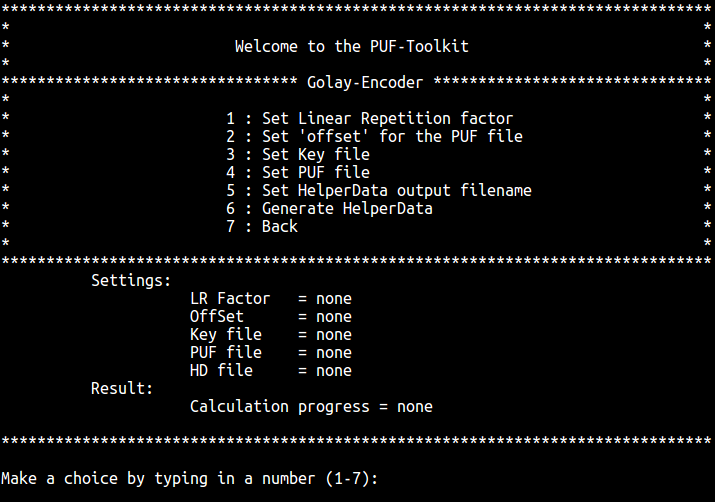
\includegraphics[width=0.9\textwidth]{images/golay_encoder_ui.png}}
	\caption{Console user interface of the \emph{PUF Golay Encoder}.}
	\label{img:golay_enc_ui}
	\end{figure}
	The UI is similar to BCH encoder but in this case we do not need to set the dimensions of the code ``n, k and d'' because Golay is a static code with the universal dimensions of (23, 12, 7) as seen in section \ref{golay_related}. The user interface is portrayed in Figure \ref{img:golay_enc_ui}, using the first option the user can set the Linear repetition factor as '7' or '15', the offsets of the PUF file can be adjusted using option two. After this it is mandatory to input the secret key filename, to be
	stored securely, and input the PUF filename to generate the helper data using fuzzy extractor algorithm, using option three and four respectively.The helper data filename is provided by the user by selecting option five. If all the inputs are satisfied and conditions are met then the helper data will be generated by choosing the last option six.\\


	\begin{figure}
	\centering
	\fbox{ \includegraphics[width=0.9\textwidth]{images/golay_encoder_functions.pdf}}
	\caption{Illustration of the Golay Encoder modules and their inter dependency.}
	\label{img:golay_enc_funcs}
	\end{figure}

	The functions of the Golay Encoder are divided into four modules similar to the BCH encoder depicted in Figure \ref{img:golay_enc_funcs}. The \emph{Setting} module contains the familiar functions ``DefineFilename'' and ``DefineSettings'' along with ``DefineOffsetlength'' which sets the value of the offsets. The \emph{View} module contains the ``ErrorMessages'' routine which is implemented in the toolkit already to check for incorrect inputs by the user and other routines to check the progress status and
	clear the screen. The \emph{Calculation} module forms the backbone of the Golay Encoder the details are listed below:

	\begin{itemize}
		\item \emph{Golay\_encode} routine's main task is to read and allocate memory for the PUF and Key file using their filenames that are given by the user. This routine then makes a call to the ``generateHelperData'' function with the initialized data members of the Item structure and memory pointers to the read files.
		\item \emph{generateHelperData} generates the encoding table using another internal function \emph{get\_syndrome} (this table is analogous to the generator matrix discussed in section \ref{golay_related} of the Golay Code) , then the secret key is encoded using the Golay Coding technique. The generated Codewords are stored in an array that undergoes the linear repetition process and finally, the LR\_Encoded codewords are XORed with the PUF response to obtain the
			helper data. The generatorHelperData stores the final output in the helperdata filename specified by the user along with the ``cfg'' settings i.e Offsets, LR factor and secret key filesize. This information will be read and used in the decoder module. Table \ref{tab:Golay_pattern} summarizes the data structure ``Pattern'' that constitute the cfg settings.

		\item \emph{get\_syndrome} function computes the generator polynomial for the corresponding (23, 12, 7) Golay code. \end{itemize}

	\begin{table}[!ht]
	\begin{center}
	\begin{tabular}{lll}
	\toprule
	\multicolumn{1}{l}{\textbf{Name}} & \multicolumn{1}{c}{\textbf{Type}} & \multicolumn{1}{c}{\textbf{Description}}\\
	\midrule
	\hline
	\emph{errorCode} & int & \multicolumn{1}{l}{\begin{tabular}[l]{@{}l@{}}Defines the utilized error correction code (0 = Golay, 1 = BCH)\end{tabular}} \\

	\emph{Golay\_BCH\_length} & int & \multicolumn{1}{l}{\begin{tabular}[l]{@{}l@{}}Defines the \emph{length} of one code word, for Golay and BCH \end{tabular}}\\

	\emph{Goly\_d\_BCH\_t} & int & \multicolumn{1}{l}{\begin{tabular}[l]{@{}l@{}}Defines for Golay the distance \emph{d} and for BCH the correction capability '\emph{t}' \end{tabular}}\\

	\emph{Golay\_k\_BCH\_m} &  int & \multicolumn{1}{l}{\begin{tabular}[l]{@{}l@{}}Defines the \emph{message length} for Golay and the parameter \emph{m} for BCH\end{tabular}}\\

	\emph{linearRep} & int & \multicolumn{1}{l}{\begin{tabular}[l]{@{}l@{}}Defines the utilized linear repetition factor\end{tabular}} \\

	\emph{puf\_offSet\_begin} & long & \multicolumn{1}{l}{\begin{tabular}[l]{@{}l@{}}Defines the starting point in a binary file (bytes to skip) from beginning \end{tabular}}\\

	\emph{puf\_offSet\_end} & long & \multicolumn{1}{l}{\begin{tabular}[l]{@{}l@{}}Defines the ending point in a binary file (bytes to skip) from the end \end{tabular}}\\

	\emph{original\_filesize} & long & \multicolumn{1}{l}{\begin{tabular}[l]{@{}l@{}}Defines the length of the original input key file \end{tabular}}\\
	\hline
	\addlinespace
	\bottomrule
	\end{tabular}
	\end{center}
	\caption{Names and types of each element in the data structure \emph{Pattern} for the \emph{PUF Golay Encoder} and a description regarding their purpose.}
	\label{tab:Golay_pattern}
	\end{table}

	A helper function \emph{SetInputLen} was implemented to aid the encoder functions in calculating the length of the file based on the offsets. This function is called internally before reading and allocating the memory for key and PUF response. It takes two arguments, first the Item structure with initialized data members as filenames and a second integer argument that point to PUF response or secret key, based on these values it calculates the input length as $input\_length =
	original\_filesize - (Offset\_end + Offset\_beginning)$. \\

	\subsubsection{Verification}
	The user interface was designed to follow the same pattern as BCH encoder to simplify the user experience. The ``Main'' module was modified to add one more menu item \emph{Golay\_Encoder\_Menu}. The merging and reuse of the existing functions was done with great care and detail to modularize the code that is suitable for further extension in the future. The verification of the consolidated code was done keeping in mind the same steps as BCH encoder:
	\begin{enumerate}
		\item The correctness of each module verified through utilization of test cases.
		\item All the possible menu options were checked and reviewed for their expected functionality
		\item Wrong inputs were tested to make sure that the toolkit accepts only legitimate inputs and display appropriate error messages to rectify the error.
		\item Unusual workflows were inspected to assess their impact on Golay Encoder functionality.
	\end{enumerate}

	Due to the static nature of the Golay Code (23, 12, 7) it can only correct up to ``three errors'' per ``twelve bits'' of the message. Consequently, this code is not suitable for encoding and large secret files. Extensive testing showed that when the resultant helper data is greater in size compared to the PUF response, the secret file is not recovered completely and via hit and trial the filesize for complete recovery of the secret key was approximated $2340$ bytes. So the recovery of ssh private keys which are
	typically greater than 3000 bytes is not possible using Golay and the user must choose the BCH fuzzy extractor instead.

	\subsection{Golay Decoder}
	The next step after encoding the secret key and obtaining the helper data is to recover the key via Golay decoding. The subtext presents the user interface and explains the procedure to restore the securely stored secret key, then the modules and functions of the decoder are illustrated. The discussion then follows the code improvement done to enhance the menu of the toolkit and finally verification strategy to check the integrated changes is shown.\\

	The user interface as shown in Figure \ref{img:golay_decoder_ui} has five main options where the user must input the helper data filename that was generated in the enrollment phase using option one. The other two mandatory options are to set the PUF response filename that is generated from the same device as used in encoding phase and to specify the output key filename where the secret key will be restored. If all the inputs are correctly set then the ``regeneration'' can be performed via option four. The output and status is displayed
	under the \emph{Result} section of the UI whereas \emph{Settings} subsection of the interface shows the filenames. If the input is incorrect or if the given filename is not present on the disk then a suitable error with details to recover from a faulty state is shown to the user.\\
	\begin{figure}
	\centering
	\fbox{ 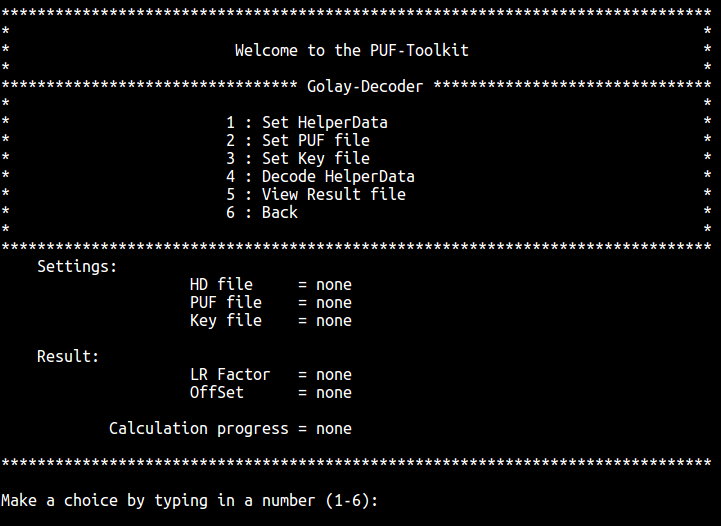
\includegraphics[width=0.9\textwidth]{images/golay_decoder_ui.png}}
	\caption{Conceptual design of the Golay Deocder user interface.}
	\label{img:golay_decoder_ui}
	\end{figure}

	\begin{figure}
	\centering
	\fbox{ \includegraphics[width=0.9\textwidth]{images/golay_decoder_functions.pdf}}
	\caption{Illustration of the Golay Decoder modules and their inter dependency.}
	\label{img:golay_decoder_fns}
	\end{figure}

	Golay decoder code is partitioned across five modules similar to the ones discussed in Golay encoder as illustrated in Figure \ref{img:golay_decoder_fns}. The first module is the Main\_Menu function that calls the Golay decoder menu. This menu was implemented and added to the PUF toolkit which on selection points to the user interface with menu items of the decoder TODO refer. The Golay Decoder user interface is implemented in the routine \emph{Golay\_Decoder\_Menu}, where the decode option is linked to the \emph{Golay\_decode}
	function that performs the decoding of the helper data. The usual routines in the ``View'' module are used to set the helper data, PUF response and output recovered key filenames. There is no need to set the offsets and original key filesize in the decoder menu since during the ``enrollment'' phase these details are appended at the end of helper data as part of the `cfg' settings. The ``Calculation'' module is crucial to the decoding operation and which follows the below-mentioned
	steps:
	\begin{enumerate}
		\item The Golay decode function reads the `cfg' settings using a subroutine \emph{read\_infos} that reads the settings appended at the end of the helper data and initializes the corresponding data members of the Item structure. The details of the data members used in Golay decoding are listed in Table \ref{tab:Golay_pattern}. Then based on the settings the input length of the PUF response is calculated as $input\_length = original\_filesize - (Offset\_end + Offset\_beginning)$. The files

			helper data and PUF response are read and stored in the memory and the control is given to the \emph{recoverOriginalData}.
		\item The next function \emph{recoverOriginalData} performs the decoding of the helper data. It first applies ``Majority Voting'' on the encoded helper data to reverse the effects of the ``Linear Repetition'' done during enrollment phase. With the help of an API \emph{next\_comb} the decoding table for Golay code (23, 12, 7) is calculated that is used to recover the original key.
		\item After the restoration of the key is complete it is saved in the output key filename by calling a
			sub-routine \emph{SaveFile} that takes the recovered key (represented in code as a character array) and output filename as arguments and uses standard C file operations to write to the file.
	\end{enumerate}

	The \emph{ErrorMessages} function was used to detect incorrect input and display the errors to the user since it is redundantly used in the other menu functionalities of the PUF toolkit like BCH encoder, we summarize the Error Codes in Table \ref{tab:Golay_dec_errors}

	\begin{table}[!ht]
	\begin{center}
	\begin{tabular}{cp{13cm}}
	\toprule
	\multicolumn{1}{c}{\textbf{Error code}} & \multicolumn{1}{c}{\textbf{Error message}} \\
	\midrule
	\hline
	1 & ERROR! Invalid input - Only digits are allowed! No digit at \emph{pos + 1}.\\

	2 & ERROR! Invalid input - Input to long. \\

	3 & ERROR! Invalid input - Try again...  \\

	4 & ERROR! Opening output file. \\

	5 & ERROR! Invalid input - 'Filename' too long. \\

	6 & ERROR! Invalid input - No input. \\

	7 & ERROR! Reading PUF file. \\

	8 & ERROR! Opening PUF file. \\

	9 & ERROR! Invalid input - PUF filename is not valid.\\

	10 & ERROR! Invalid input - Key filename is not valid.\\

	11 & ERROR! Opening HelperData file. \\

	12 & ERROR! Reading HelperData file. \\

	13 & ERROR! Selected an invalid choice. \\

	14 & ERROR! HelperData: The recovered 'decoding information' is invalid! -> Parameter '\emph{m}' is out of range.\\

	15 & ERROR! HelperData: The recovered 'decoding information' is invalid! -> Parameter '\emph{t}' is out of range.\\

	16 & ERROR! HelperData: The recovered 'decoding information' is invalid! -> Parameter '\emph{length}' is out of range.\\

	17 & ERROR! HelperData: The recovered 'decoding information' is invalid! -> Parameter '\emph{LR factor}' is not 7 or 15.\\

	18 & ERROR! HelperData: The recovered 'decoding information' is invalid! -> Parameter '\emph{offSet}' is out of range.\\

	19 & ERROR! HelperData: The recovered 'decoding information' is invalid! -> Parameter '\emph{filesize}' is out of range.\\

	20 & ERROR! Opening file to view.\\

	21 & WARNING! Looks like no decoding was performed.\\

	22 & Looks like the calculation was not started.\\

	23 & ERROR! Looks like the file was empty.\\

	24 & ERROR! Looks like the file was not in the supported format.\\

	25 & WARNING! Looks like the 'offset' is not set.\\

	26 & ERROR! Looks like the 'Output file or Result' is not set/calculated.\\
	\addlinespace
	\bottomrule
	\end{tabular}
	\end{center}
	\caption{Error codes and corresponding error messages for the \emph{PUF Golay Decoder}.}
	\label{tab:Golay_dec_errors}
	\end{table}

	\subsubsection{Verification}
	After the merging is complete and the Golay decoder menu is functional it was tested rigorously to make sure all the options work as expected. The same approach for verification was taken as mentioned in previous subsections and a final check was done to compare the recovered key with the original secret to ensure the overall functionality of both the Golay Encoder and Decoder is correct.

	\begin{itemize}\itemsep-\the\parsep
		\item Every menu item of the Golay Decoder was checked and review to make sure it behaves as expected.
		\item Incorrect inputs were inserted deliberately to verify the ErrorMessages routine display corresponding error messages and ways to recover from the incorrect state of the toolkit.
		\item Unusual workflows were inspected to assess their impact on Encoder functionality.
		\item The recovered key was compared with the original secret key via the Linux ``diff'' command line utility and they were found to be identical.
	\end{itemize}

	\section{Jaccard Index}
	\label{jaccardi_index_section}
	This section explains the Jaccard Index implementation that was developed as a new feature for the toolkit. Then the two sub-menu options Intra Jaccard and Inter Jaccard Index are presented as subsections.
	The modules and code structure was inspired from the Hamming Distance Menu since both of the metrics (Hamming Distance and Jaccard Index) are closely related to each other and operate on either files or folders. We first discuss the definition of Jaccard Index and its relation to the hamming weight. We then look at the user interface for the Jaccard Index Menu which contains two more sub-menu options \emph{Inter} and \emph{Intra Jaccard index} and then go on to explain the modules of the
	Jaccard index. In the end, the section presents the verification steps after the development of this new feature was complete.\\

	\begin{itemize}
		\item \textbf{Definition}: Jaccard index between two bytes A and B is defined by the Equation \ref{jaccard_eq}
		\begin{equation}
		J(A,B) = \frac {|A \cap B|} {|A\cup B|} = \frac{|A \cap B|} {|A| + |B| - |A \cap B|}
		\label{jaccard_eq}
		\end{equation}
		where |A| is the hamming weight of A, |B| is the hamming weight of B and $|A \cap B|$ is the number of times both A and B have one in the same bit position.
	\end{itemize}

	For eg. if we have two bytes A = 1100 1111 and B = 1111 0000 then |A| = 6, |B| = 4 and $|A \cap B|$ = 2 (since only first two common positions have ones in both the bytes). Substituting these values in the above equation we get $J(A,B) = (2) / ( 6 + 4 - 2) = 0.25$.\\

	\begin{figure}[h]
	\centering
	\fbox{ 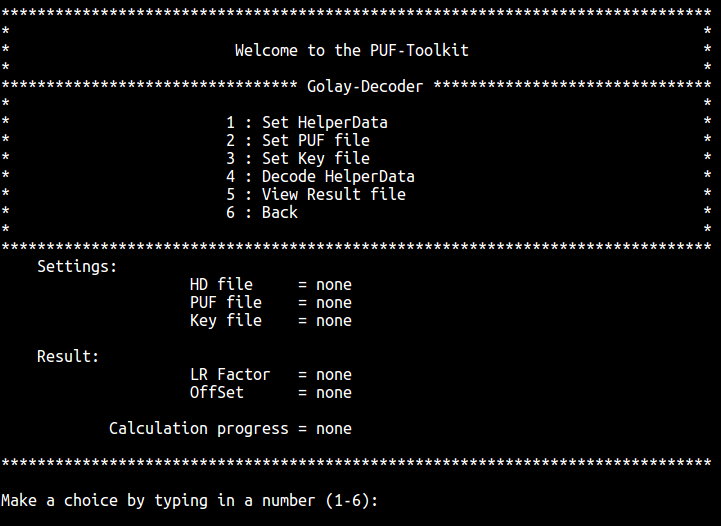
\includegraphics[width=0.9\textwidth]{images/golay_decoder_ui.png}}
	\caption{Conceptual design of the Jaccard Index user interface.}
	\label{img:jaccard_ui}
	\end{figure}
	The user interface for the Jaccard Index menu is similar to the Hamming Distance Menu as shown in Figure \ref{img:jaccard_ui}. Using the first option user can set the offsets from beginning and end of the file and as a result, those bytes will be skipped during Jaccard calculation. The second option lets the user set the output filename which is mandatory since the results will be stored in this file. The third option performs the computation of the Jaccard index between the two given
	files. It first asks for the two filenames to be prompted by the user and then the result along with the \emph{Fractional Index} is stored in the output file. Option five and six calls the Intra and Inter Jaccard Index routines respectively and are discussed in following subsections. The six and the last option can be used to view the output file without exiting the toolkit.\\

	The modules of the Jaccard's index are similar to those of the Hamming Distance and therefore this section takes the liberty of not showing it here again.
	Rather than looking at each and every module, we look at the main routines and algorithm to calculate the Jaccard Index.
	\begin{itemize}
		\item The main Jaccard index between two files is calculated by the \emph{Jaccard\_Index} that takes data structure Item pointer as an argument with initialized filenames. It first sets the input length of both the files based on the offsets from beginning and end by calling the \emph{SetInputLen} API which was designed specifically for this purpose.
		\item Then the files are read using the sub-routine \emph{readfile} that takes the name of the file, offset from beginning and filesize as an argument, based on that it reads and mallocs the file in memory and passes back the pointer to the allocated memory back to the caller function.
		\item To get the common number of ``1s'' at same bit positions in both the files, a bitwise AND operation is performed on the read files and the result is stored in a character array. The resultant character array contains the data with ``1s'' in the same bit position since bitwise AND operation only yields result ``one'' both the input bits are ``one''. This operation can be seen in Table \ref{bitwise_AND}.

	\begin{table}[!ht]
	\begin{center}
	\begin{tabular}{lc}
	\toprule
	\multicolumn{2}{c}{\textbf{bitwise AND of two bytes A and B}}\\
	\midrule
	Byte A &   1100 0000 \\
	Operation & \&\\
	Byte B &   1111 0011 \\
	Output C &   1100 0000 \\
	\addlinespace
	\bottomrule
	\end{tabular}
	\end{center}
	\caption{bitwise ANDing the two bytes to get the common ones in the same bit position}
	\label{bitwise_AND}
	\end{table}

		\item Once the bitwise AND result is obtained then the calculation of Jaccard Index is relatively simple. The number of ones in each input files and the bitwise ANDed output file are computed by calling the \emph{hamming\_wt} function explained in section \ref{Hamming_Distance_menu} under listing \ref{lst:hammingwt} and then the values are substituted in the Equation \ref{jaccard_eq}.
	\item An additional metric called Fractional Jaccard's Index is also calculated using the definition $F(A, B) = J(A, B)/ size(A or B)$ and written to the result file along with the Jaccard Index.
\end{itemize}

\subsection{Intra Jaccard Index}
Instead of computing Jaccard index between two files, the entire folder containing PUF responses from a single device can be evaluated by selecting the Intra Jaccard Index sub-menu item. The filename where the results will be written is essential before processing the Intra Jaccard Index. The menu item asks for an input directory with a relative or absolute path on the machine and if the input path is correct and an output file is set then the result is generated and stored in the
output file.\\

Contrary to the intra hamming distance the ``Switch output-style'' (refer section \ref{intra_hd_section}) option was not made available to the user to simplify the functionality. The default output-style was set as \emph{Compact} which is explained in detail in the Intra Hamming Distance section \ref{intra_hd_section} and illustrated in Figure \ref{img:4_intra_WP}. A sample result output file is presented in Figure \ref{img:intra_jaccardi_compact} which shows the compact mode comparison between the files in the
directory where the Jaccard Index in conjunction with fractional Jaccard Index is written for each comparison.\\

\begin{figure}[h]
\centering
\fbox{ \includegraphics[width=0.9\textwidth]{images/intra_jaccardi.pdf}}
\caption{A sample output result showing the \emph{compact} output style format for Intra Jaccard Index }
\label{img:intra_jaccardi_compact}
\end{figure}

To realize the Intra Jaccard Index the function \emph{Jaccard\_Intra} was implemented that takes the directory as input and first checks if the path is valid and there are more than one files present in the folder. Then all filenames with their absolute paths are stored in a standard C++ vector data structure. The \emph{Jaccard\_Intra} then iterates through this vector and computes the Jaccard Index for each comparison by calling the \emph{Jaccard\_Index} procedure that was explained in  section
\ref{jaccardi_index_section}
above. Finally, the result is written in each iteration of the loop and appended to the output file.\\

\subsection{Inter Jaccard Index}
Unlike its Intra counterpart, the Inter Jaccard Index can be used to evaluate the PUF responses across different devices. It compares the PUF responses in a directory (analogous to a device since all PUF responses from a single device are stored in the same folder) to PUF responses in other directories. The comparison mode or the output-style by default is designed in the code to be ``compact'' since it simplifies the metric and also avoids any duplicate comparisons. The details of
the compact mode file comparison for Inter Jaccard index are the same as for Inter Hamming Distance which is explained in detail in section \ref{inter_hd_section} and the  compact comparison operation between three folders is shown in Figure \ref{img:inter_compact}.\\

The code implementation for Inter Jaccard Index is achieved by the routine \emph{Jaccard\_Inter} which takes the data structure Item as an argument. The user needs to input the number of paths or folders he/she wants to evaluate, this number is bounded between \emph{two} and \emph{ninety-nine} i.e $2 <= n < 99$, then the folder names with their absolute or relative path are required by the toolkit. All these paths are verified by the code as valid and present in the memory, the
routine \emph{Jaccard\_Inter} verifies if each given folder has at least one file. These folder names and paths are then stored in a standard C++ vector which is navigated in compact comparison fashion to compute the Jaccard Index. The nested for loop iterations are abstracted in this text to avoid complexity. In each iteration of the nested loop the comparison between PUF responses of different devices is achieved by redundant calls to the \emph{Jaccard\_Index} function explained in section
\ref{jaccardi_index_section} and result is written to the output file as specified by the user.\\

\subsection{Verification}
The merging of a new feature to the toolkit required careful testing to ensure correctness and exceptions to be handled gracefully. Some of the approaches were inspired from the fuzzy extractor testing and are summarized below:
\begin{itemize}
	\item All the menu item were checked and reviewed for their expected functionality.
	\item Testing was done for faulty and incorrect inputs to the Jaccard Index menu options to ensure relevant error messages are displayed to the user. For eg., incorrect paths or filenames of the directories will be prompted to the user suggesting to enter the paths/filenames again.
	\item The Jaccard output file was reviewed to check for proper header information and tables.
	\item For Intra and Inter Jaccard index, the mandatory options like setting of the offsets and the output file was checked before computing the index. In case these settings are not configured then relevant error information was displayed to the user.
\end{itemize}

This marks the completion of the improvement and development phase of the toolkit. Next part of the report discusses the integration of the toolkit to the CogniCrypt opensource library by interfacing the C++ APIs to the Java runtime via Java Native Interface.

\section{CogniCrypt Integration}

To make the C++ source code functions available to the Java runtime they must be interfaced using the Java Native Interface Technology. This section looks at the details of the Java Native interface, most of which is inspired from \cite{jni}, then the code implementation for the JNI is explained. Next, the wrapping procedure of the toolkit as a shared library and packaged as a Java Archive (JAR) to be externally linked by the Java source code is clarified. The next subsections describe the Congicrypt and its clafer model
along with the XSL coding techniques to generate the Java biolerplate code to assists the Java developers.

\subsection{Java Native Interface}
Java Native Interface standard and programming techniques are defined by Oracle\textsuperscript{TM} as a native programming interface which allows Java code that runs inside a Java Virtual Machine (VM) to interoperate with applications and libraries written in other programming languages, such as C, C++, and assembly. The JNI does not impose any restriction on the implementation of the underlying Java Virtual Machine so the native code works irrespective of the Virtual machine.\\

To implement the JNI code a lot of help was taken from the tutorial \cite{jni_tutorial}, for each metric of the toolkit an API was designed in accordance with the syntax of the JNI. The text explains the development process for a single metric Hamming Distance, these steps are applied to all the other metrics too. The toolkit.java source file was written containing the native interfaces to the functions in the PUF toolkit. For eg., Hamming weight functionality of the toolkit was available via a
public \emph{native} Java function \emph{hammingwt} that takes ``file/folder name'', ``output filename'' and ``mode''(file mode or folder mode) as arguments.  These native APIs are the class member functions of the Java \emph{toolkit} class.\\

The compilation of the toolkit Java source was performed resulting in the toolkit.class file. Next, the header file to be included in the JNI C++ source code was generated using the ``javah'' utility. The resultant header file contains the syntactical prototypes of the C++ interface functions that must be implemented. Such a file with hamming distance metric is shown in listing \ref{lst:jni_header}.
\begin{lstlisting}[frame=single,language=C++,
commentstyle=\color{magenta},
backgroundcolor=\color{white},
keywordstyle=\color{blue},
stringstyle=\color{orange},
basicstyle = \ttfamily \color{black} \footnotesize,
caption={Auto generated header file showing the syntax for Java Native Interface function declarations} ,
label={lst:jni_header},
captionpos=b,
numbers=left]
/* DO NOT EDIT THIS FILE - it is machine generated */
#include <jni.h>
/* Header for class jni_toolkit */

#ifndef _Included_jni_toolkit
#define _Included_jni_toolkit
#ifdef __cplusplus
extern "C" {
#endif
/*
 * Class:     jni_toolkit
 * Method:    hammingwt
 * Signature: (Ljava/lang/String;Ljava/lang/String;Z)V
 */
JNIEXPORT void JNICALL Java_jni_toolkit_hammingwt
  (JNIEnv *, jclass, jstring, jstring, jboolean);
\end{lstlisting}

The \emph{Java\_jni\_toolkit\_hammingwt} interface first parses the arguments that it obtained from the Java source code. It takes the jstring arguments file/folder name and output filename and converts them into standard C character array using the standard JNI conversion function \emph{GetStringUTFChars}. The jboolean argument is implicitly an integer so it does not require any transformation. The code then initializes the ``Item'' data structure with these values and calls the \emph{HammingWeight(Item *, int )} function of the toolkit to compute the hamming distance of the file or the entire folder based on the value of $mode$.\\ 

The \emph{ErrorMessages} routine of the toolkit is used to inform the user about invalid inputs and faulty toolkit states. Since these inputs are passed from the Java source as strings, the Java developers can check at their end for the authenticity of the file/folder names and their path on the machine. Other metrics of the PUF toolkit like ``entropy'', ``median and average'' etc. are implemented similarly in the Java source and C++ source code.\\

\subsubsection{Packaging in Java Archive}
The C++ JNI source code along with the entire PUF toolkit must be compiled and linked as a shared library since the Java source code calls the native functions from the shared library or shared object. Before packaging the shared library and other Java-related class files in a JAR file the toolkit must be compiled as a shared object file. This is achieved by compiling and linking the PUF toolkit with the
``-fPIC'' and ``-shared'' flag of the GNU g++ compiler. The resultant ``libtoolkit.so'' can then be packaged in a JAR file.\\

JNI standard provides the API \emph{System.loadLibrary} to load the shared objects or Dynamic-Link Libraries (DLL) from the Java source code, but the CogniCrypt project requires the shared library and the Java toolkit.class to be packaged in a JAR , so that they can be included in the project as an External Library. For this purpose, another class is needed that can extract the shared object from the JAR , load it using the standard JNI function and then delete before the Java runtime exits. Such
a wrapper class was already implemented and after little changes, it was tailored to meet the needs of this project. To know more details about the implementation of this Java source please refer \cite{nativeutils}.\\

Once the toolkit.class, NativeUtils.class and libtoolkit.so are compiled they are packaged as a JAR file which is exported in the CogniCrypt as an External Archive.

\subsection{CogniCrypt Clafer Model}
CogniCrypt was implemented as an Eclipse Plugin to support the Java developers to enable easier use of the Cryptographic APIs \cite{cogni}. It helps the developers to:
\begin{itemize}
	\item Generate secure implementations for cryptographic tasks like Data Encryption.
	\item Analyzes the Java code and alerts for insecurely used cryptographic APIs.
\end{itemize}

CogniCrypt supports various crypto tasks and for the PUF toolkit to be made available on the list, a new task ``Evaluation and Assessment of PUF responses'' was implemented. After selecting the task a few high-level questions like if the developer wants to evaluate PUF response from a single or multiple devices as shown in Figure \ref{img:cogni_ques}, must be answered by the developers.\\

\begin{figure}[h]
\centering
\fbox{ 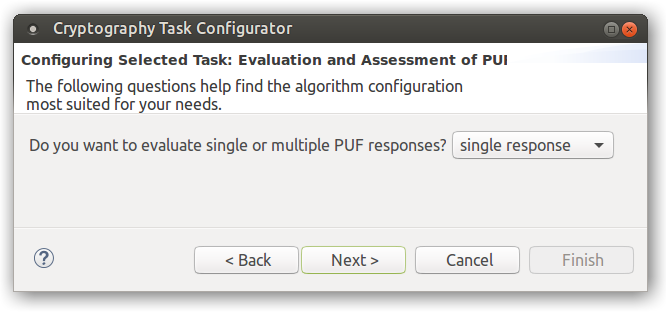
\includegraphics[width=0.9\textwidth]{images/Cogni1.png}}
\caption{An example of High level questions asked by the CogniCrypt for the Evaluating PUF responses}
\label{img:cogni_ques}
\end{figure}

Once all the questions are acknowledged, based on their answers the CogniCrypt presents a list of the algorithms that are eligible for selection for e.g if the developer answered evaluation of PUF response from ``multiple devices'' then Inter Hamming Distance is only shown in the drop-down since it is the only metric in the toolkit that takes more than one directory as input. In this case, the CogniCrypt generates a Java boilerplate code that shows the proper usage of the Inter Hamming Distance
function of the toolkit with directories (bounded between 2 and 99) as parameters to the API.\\

To achieve the above-mentioned functionality the CogniCrypt employs a Clafer based model which is a lightweight modeling language that facilitates a mix of class and feature modeling \cite{clafer,cogni}. It supports constraint solvers that can generate instances of a model and satisfy its constraints \cite{cogni}. The answers to the high-level questions determine the constraints on the model which is composed of different elements known as clafer. For the PUF toolkit each evaluation metric was

\begin{lstlisting}[frame=single,language=C++,
commentstyle=\color{magenta},
backgroundcolor=\color{white},
keywordstyle=\color{blue},
stringstyle=\color{orange},
basicstyle = \ttfamily \color{black} \footnotesize,
caption={Code snippet of a sample metric Hamming Distance in the PUF clafer model} ,
label={lst:pufcfr},
captionpos=b,
numbers=left]
abstract Metric
	description -> string
	fileMode -> FileMode
	devices -> Devices

Hamming_Distance : Metric
	[description = "hamming distance"]
	[fileMode = File || fileMode = Folder]
	[devices = Single]
\end{lstlisting}

The hamming distance extends the abstract Metric class that has two enums ``filemode and devices'', and a string element as data members. These elements are initialized in the \emph{Hamming\_distance} class, lines 11-12 make ensures the hamming distance can only be evaluated for a file or an entire folder, such conditions are applied to other metrics too, for eg., Inter Hamming distance must always evaluate for multiple devices.\\ 

After the clafer model is finalized and implemented, auto-generation of the Java code, that shows the developers the correct usage of the PUF toolkit functions, is achieved by the XSL stylesheet. For the PUF Toolkit the already implemented stylesheet in the CogniCrypt was enhanced to support the new functionality. Based on the answers by the developer to the high-level questions the algorithm type or the metric is set in the clafer model which can be used by the <xsl: if> statements
to match and generate appropriate usage sample code. %For eg. listing \ref{ } shows the XSL stylesheet code to match the Hamming Distance metric and consequently produce java code that shows its proper usage.


